\documentclass{article}
\usepackage{amsmath,amssymb,amsthm,kotex,paralist,mathrsfs,url,hhline}

\newcounter{num}[section]
\newcommand{\defi}[1]
{\bigskip\noindent\refstepcounter{num}\textbf{정의 \arabic{num}) #1}\par}
\newcommand{\theo}[1]
{\bigskip\noindent\refstepcounter{num}\textbf{정리 \arabic{num}) #1}\par}
\newcommand{\axio}[1]

\begin{document}
\title{현빈 : 11 이차부등식}
\author{}
\date{\today}
\maketitle

%\defi{이차방정식}
%\(a\), \(b\),\(c\)가 실수이고 \(a\neq0\)일 때, 방정식
%\[ax^2+bx+c=0\]
%을 \emph{이차방정식}이라고 부르고, 이 식을 만족시키는 \(x\)의 값을 이 이차방정식의 \emph{근} 또는 \emph{해}라고 부른다.
%여기에서는 \(a>0\)인 이차방정식만을 다룬다.
%
%\theo{이차방정식의 근의 위치 판별 조건}
\(a\), \(b\), \(c\)가 실수이고 \(a>0\)일 때 이차부등식 \(ax^2+bx+c>0\), \(ax^2+bx+c\ge0\), \(ax^2+bx+c<0\), \(ax^2+bx+c\le0\)의 해는 다음과 같이 구해진다.
\bigskip

\noindent
{\footnotesize
\begin{tabular}{p{0.24\textwidth}|p{0.24\textwidth}|p{0.24\textwidth}|p{0.24\textwidth}}
\hline
&\(D>0\)		&\(D=0\)	&\(D<0\)\\
\hline
이차함수의 그래프
&\raisebox{-.5\height}{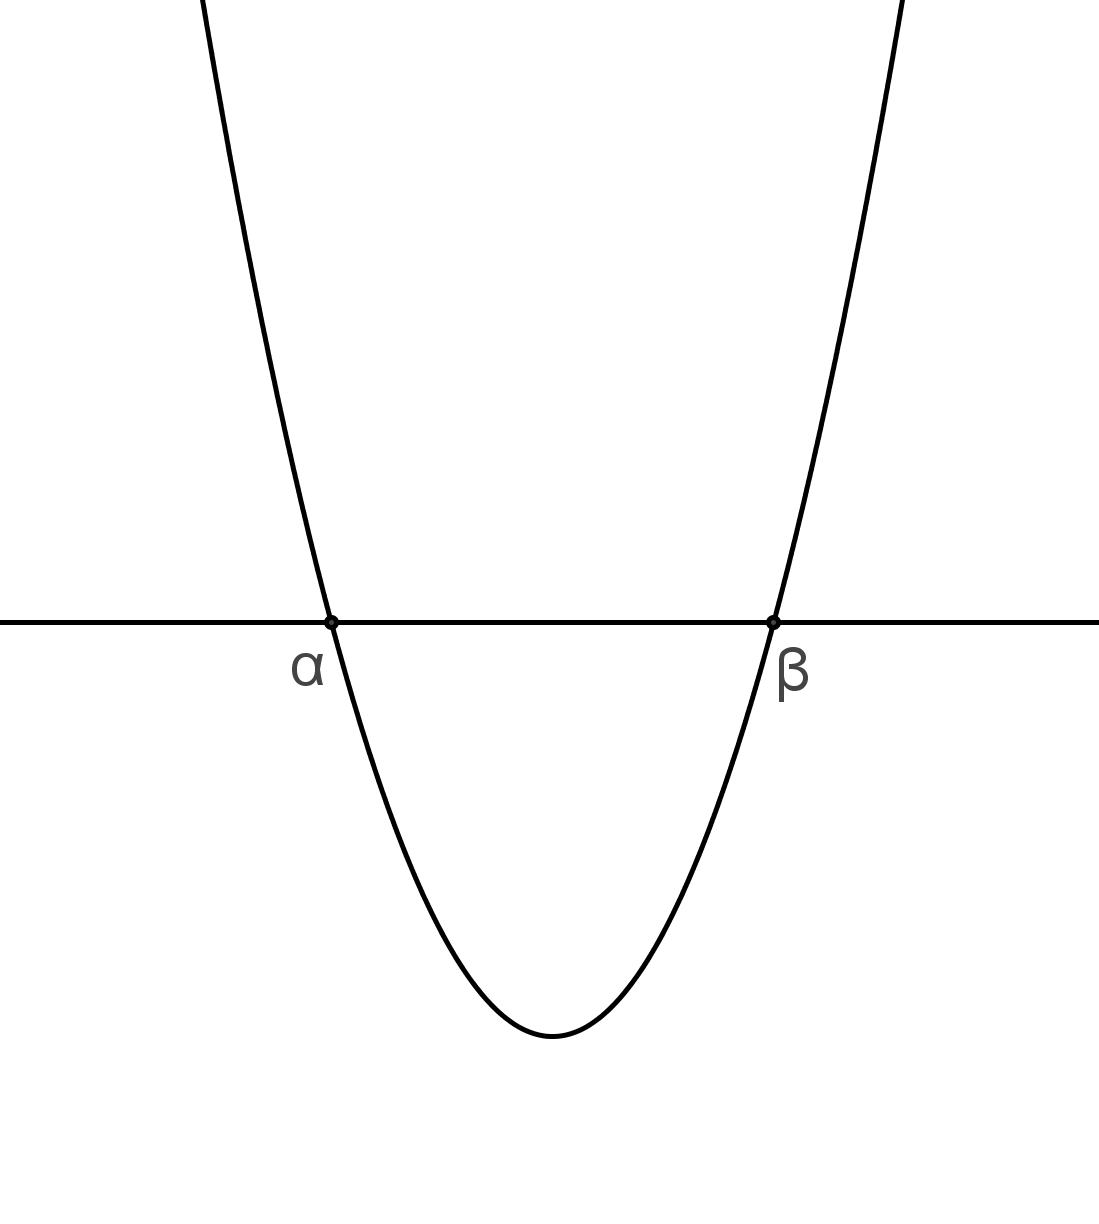
\includegraphics[width=0.24\textwidth]{1}}
&\raisebox{-.5\height}{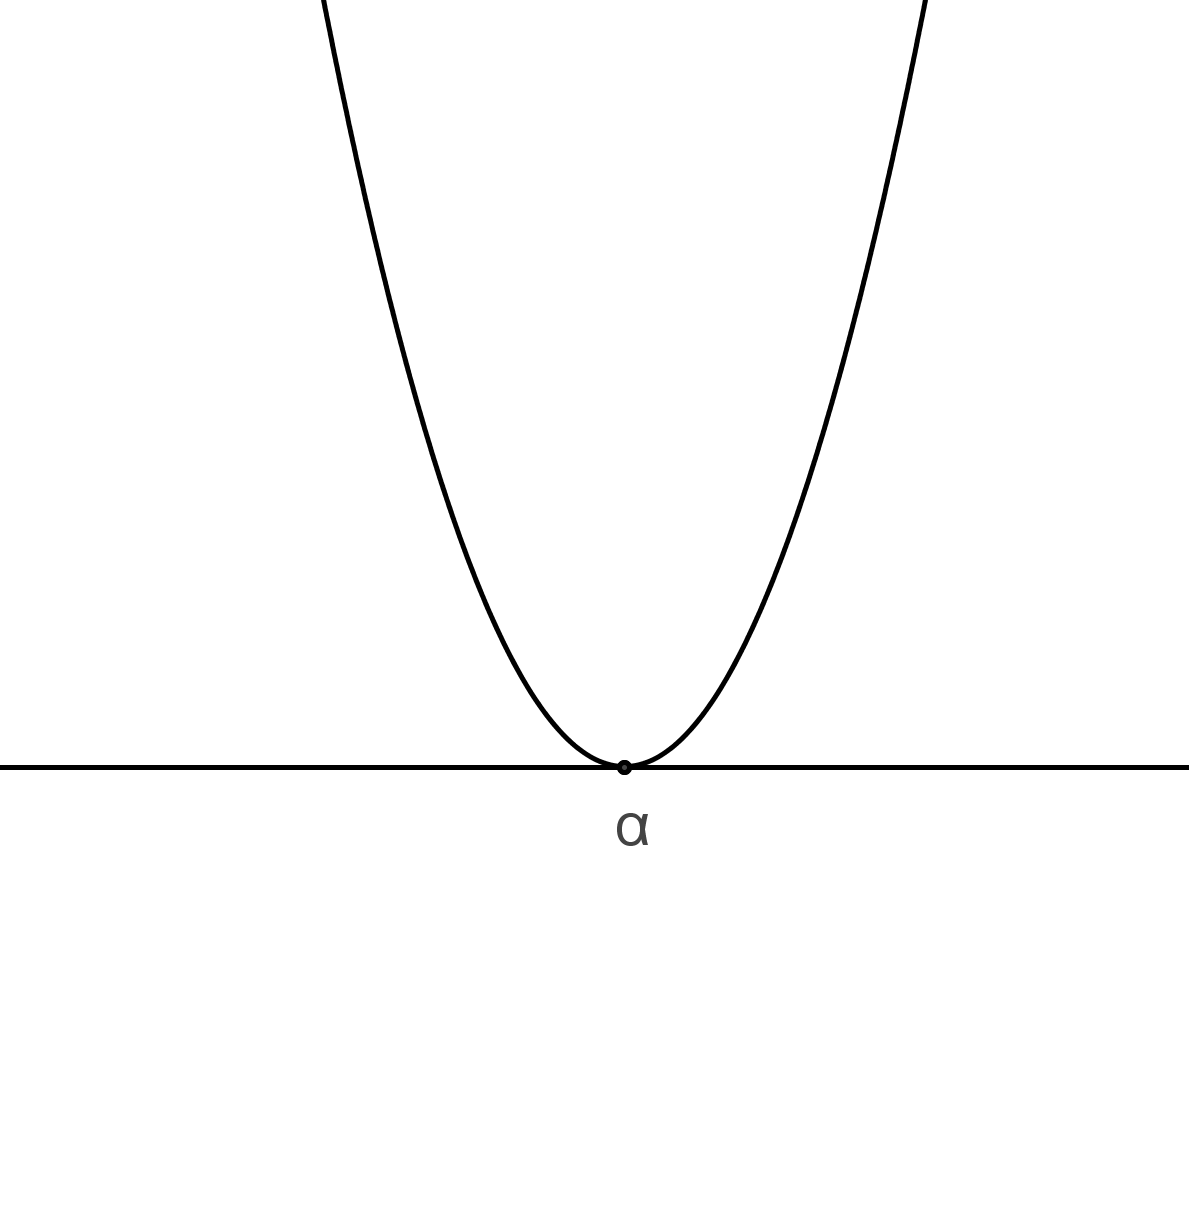
\includegraphics[width=0.24\textwidth]{2}}
&\raisebox{-.5\height}{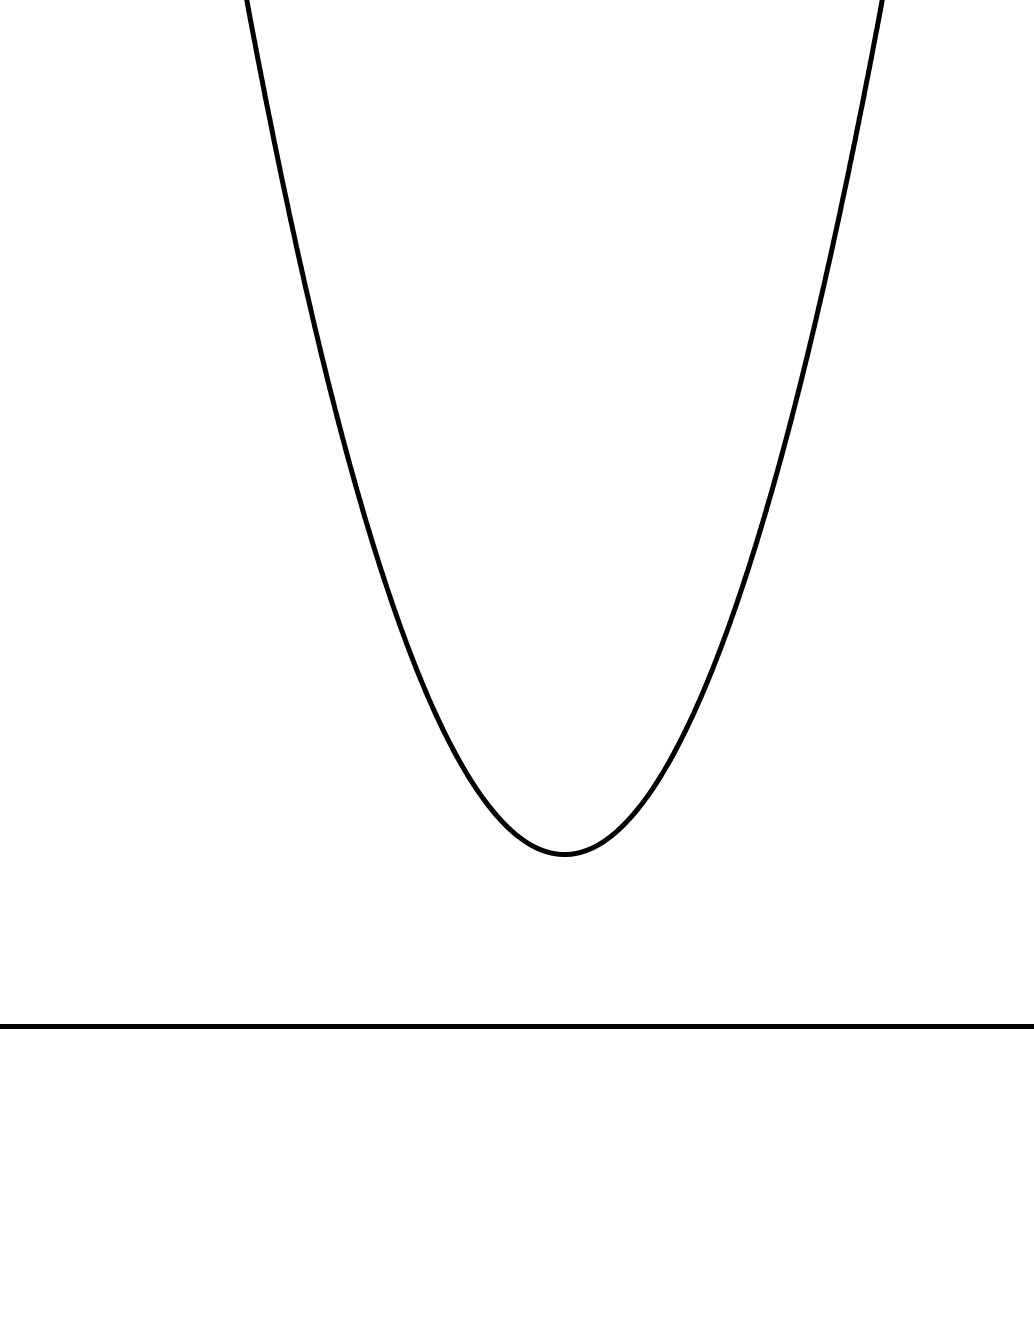
\includegraphics[width=0.24\textwidth]{3}}\\
\hline
\(ax^2+bx+c>0\)의 해
&\(x<\alpha\) 또는 \(x>\beta\)		&\(x\neq\alpha\)인 모든 실수	&모든 실수\\\hline
\(ax^2+bx+c\ge0\)의 해
&\(x\le\alpha\) 또는 \(x\ge\beta\)	&모든 실수					&모든 실수\\\hline
\(ax^2+bx+c<0\)의 해
&\(\alpha<x<\beta\)				&없다.					&없다.\\\hline
\(ax^2+bx+c\le0\)의 해
&\(\alpha\le x\le\beta\)			&\(x=\alpha\)				&없다.\\\hline
\end{tabular}
}

\newpage
--------------------- 예 제 ---------------------

09.
이차함수의 그래프를 이용하여 다음 이차부등식을 풀어라.

\quad\:
(1) \(-x^2+4x+5\ge0\)

\quad\:
(2) \(x^2-4x+4>0\)

\bigskip
11.
다음 이차부등식을 풀어라.

\quad\:
(1) \(x^2-x-2<0\)

\quad\:
(2) \(x^2\ge2x+4\)

\quad\:
(3) \(-x^2+x+6\le0\)

\bigskip
12.
다음 이차부등식을 풀어라.

\quad\:
(1) \(x^2+4x+4>0\)

\quad\:
(2) \(64\le16x-x^2\)


\bigskip
13.
다음 이차부등식을 풀어라.

\quad\:
(1) \(x^2+x+1>0\)

\quad\:
(2) \(5x\ge x^2+9\)

\bigskip\bigskip
--------------------- 연습 문제 ---------------------

207.
이차함수의 그래프를 이용하여 다음 이차부등식을 풀어라.

\quad\:
(1) \(x^2-6x+8\le0\)

\quad\:
(2) \(x^2-4x+5<0\)

\quad\:
(3) \(4x^2-4x+1\le0\)

\bigskip
209.
다음 이차부등식을 풀어라.

\quad\:
(1) \(2x^2-3x-2>0\)

\quad\:
(2) \(x^2-x-12\le0\)

\quad\:
(3) \(-x^2+6x+3\ge0\)

\quad\:
(4) \(3x^2-5x-2\le0\)

\quad\:
(5) \(x^2-4x+2\ge0\)

\bigskip
210.
다음 이차부등식을 풀어라.

\quad\:
(1) \(x^2-6x+9>0\)

\quad\:
(2) \(x^2-x+3<0\)

\quad\:
(3) \(x^2-2x+4>0\)

\quad\:
(4) \(2x^2+2x+3>0\)

\quad\:
(5) \(4x^2-12x+9\le0\)

\quad\:
(6) \(-2x^2+8x-9\ge0\)

--------------------- 추가 문제 ---------------------

227.
다음 이차부등식을 풀어라.
\quad\:
(1) \(-3x^2+4x+15<0\)

\quad\:
(2) \(x^2+4x-3\le0\)

\quad\:
(3) \(x^2-10x+24<0\)

\quad\:
(4) \(4-x^2<0\)

\quad\:
(5) \(2x^2\ge x+6\)

\quad\:
(6) \(-3x^2+8x-2\ge0\)

\bigskip
228.
다음 이차부등식을 풀어라.
\quad\:
(1) \(-x^2+6x+9\ge0\)

\quad\:
(2) \(x^2+8x+16\ge0\)

\quad\:
(3) \(-9x^2\ge4-12x\)

\quad\:
(4) \(4x^2-12x+9>0\)

\bigskip
229.
다음 이차부등식을 풀어라.
\quad\:
(1) \(-x^2+2x+3>0\)

\quad\:
(2) \(-2x^2+3x-6\ge0\)

\quad\:
(3) \(2x^2+3x+4>0\)

\quad\:
(4) \(3x^2-2x+1\ge0\)

\bigskip
236.
이차부등식 \(x^2+ax+b\le0\)의 해가 \(x=3\)뿐일 때, 실수 \(a\), \(b\)의 합 \(a+b\)의 값을 구하여라.

\bigskip
237.
어떤 실수 \(k\)에 대하여 이차부등식 \(x^2+ax+a+3>0\)의 해가 \(x<k\) 또는 \(x>k\)일 때, 다음 중 \(a\)의 값이 될 수 있는 것은?


\end{document}